\section{Bilateral Filter}


The depth maps captured by a low cost RGB-D camera usually contains noise, this can be 
consequence of materials reflectance, device imperfections, object fast movement, distance to the 
sensor, etc. 

In order to reduce the effect of noise is natural to use some kind of filter, as usual in computer 
vision, a typical filter will take information of a pixel and its neighborhood to generate a result. 
If the image is smooth, without abrupt changes in intensity, a simple average could be enough. However, this 
is not the case in the presence of edges or corners, areas where the intensity changes sharply. 
The bilateral filter deals this problem, giving to each neighbor a weight based on its closeness  
to the center pixel. In a grayscale image it takes into account 
the neighbor intensity distance and location distance (in image plane) to calculate the weight.  A depth map is very similar to a grayscale 
image, the only difference is that the depth map represents geometrical information (3D points) and usually contains holes 
(areas where the sensor failed to measure distance). 

A bilateral filter was applied to the depth maps, using the euclidean distance and the distance along the $z$ axis to calculate 
the weight of each pixel neighbor in the depth map. 

In a filter window centered at a 3D point $p$, corresponding to one depth map pixel, 
the weighted average was calculated using the following weight for each neighbor:


$$ w(p,q,\sigma_d,\sigma_z) = k(d(p,q),\sigma_d) k(z(p,q),\sigma_z)\ , $$

\noindent where 

$$ k(v,\sigma) = \frac{e^{-v^2}}{2*\sigma^2}\ , $$
$$ d(p,q) = ||p - q||\ , $$
$$ z(p,q) = |p_z - q_z|\ , $$
$$ p = (p_x,p_y,p_z)\ , $$ 
$$ q = (q_x,q_y,q_z)\ . $$

\noindent $p$ is the central point 3D coordinate and $q$ the 3D coordinate of one of its neighbors. 3D coordinates are obtained using
 the depth map and equations \ref{eq:depthmapx} and \ref{eq:depthmapy}.  Each point has a weight that depends on its euclidean distance and
 the distance along the $z$ axis, to the central point. The parameter $\sigma_d$ defines 
the neighborhood, all points of the depth map that are at euclidean distance $2*\sigma_d$ or less from the central point are considered, the 
central point itself also is considered as part of the neighborhood.


Let 


$$ W = \sum\limits_{q\ \in\ p\ neighborhood} {w(p,q,\sigma_d,\sigma_z)}\ ,$$

\noindent the final value of the central pixel of the depth map that corresponds to the 3D point $(p_x,p_y,p_z)$ is then

$$p_z' = \frac{1}{W}\sum\limits_{q\ \in\ p\ neighborhood}{w(p,q,\sigma_d,\sigma_z)q_z}\ ,$$


After applying this filter we obtain a smoothed version of the depth map, without loosing edges and important geometrical information.
A detailed explanation of the bilateral filter can be found in \cite{TomasiBilateral}.

\begin{figure}[h!]
\begin{center}
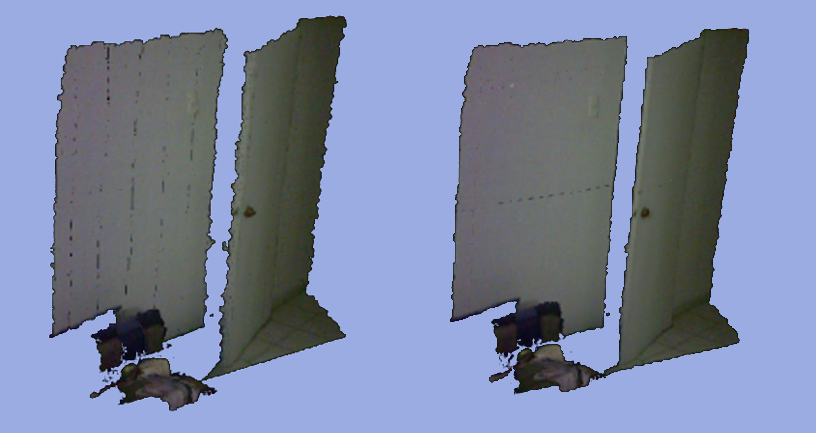
\includegraphics[scale=0.35]{images/bilateral}
\end{center}
\caption{Left: point cloud without filtering. Right: point cloud with bilateral filtering. Noticeable effects at first sight next to the borders of objects}
\end{figure}

